\documentclass[fleqn,10pt]{olplainarticle}
% Use option lineno for line numbers 

\title{Medical Code Prediction from Clinical Text with BERT}

\author[1]{Ryan Connelly}
\author[2]{Nabeel Nauman}
\author[3]{Benjamin Wang}
\author[4]{Evgeny Zolotarev}
\affil[1]{rconnelly3@gatech.edu}

\affil[2]{nabeelnau@gmail.com}
\affil[3]{bwang421@gatech.edu}
\affil[4]{ezolotarev3@gatech.edu}



\keywords{Machine Learning, BERT, Medical Code Prediction}

\begin{abstract}
The International Classification of Diseases (ICD) is an international, standardized health care classification system that maps procedures and diagnoses to alphanumeric codes. These codes allow for more consistent and accurate health information and are used for medical research, billing purposes, funding requests, and other healthcare-related activities. Currently, the process of mapping ICD codes to patient’s records is heavily manual, requiring hospital employees to read through records in depth to apply the correct codes. With such a time-consuming process, even an expert-level understanding of the thousands of ICD codes can result in incomplete or inaccurate mappings.

The ability to successfully automate ICD coding will combat issues associated with manual coding and ultimately increase the value of healthcare data.

In this paper, we explore possible improvements to previous work in this domain, namely the CAML model created by Mullenbach et al. This is done by applying Bi-Directional Encoder Representations from Transformers (BERT), a powerful language representation model released by Google AI's research team, to predict ICD-9 codes from patient discharge summaries from the MIMIC-III database. 

Our preliminary results with BERT model showed that it slightly underperforms the CAML model. We achieved 90% evaluation accuracy and 0.85 Micro-F1 score on a reduced, top 50 label set only using sequences with a maximum length of 128.  However, we expect better results when we increase the maximum length to 512.

\end{abstract}

\begin{document}

\flushbottom
\maketitle
\thispagestyle{empty}

\section{Introduction}

Mapping of ICD-9 codes is a critical step to clinical practices, particularly in the setting of intensive care units (ICUs) where the level of attention and medical care provided is far superior to regular visits \cite{mortalityPredictionUsingFuzzyClassifier}. Besides streamlining treatment, ICD-9 codes have a variety of other uses such from billing to building predictive models of the patient’s current and future state \cite{nlpProcessingForClinicalDecisionSupport}.

Scheurwegs et al. \cite{scheurwegsSelectingRelevantFeaturesFromEHR} used a feature selection approach to ICD-9 and ICD-10 classification, incorporating both MIMIC-III and various medical ontologies.

Mullenbach et al. in Explainable Prediction of Medical Codes from Clinical Text \cite{explainablePredictionMedicalCodes} were able to achieve better accuracy with only the MIMIC-III dataset by developing the Convolutional Attention for Multi-Label classification (CAML) method. CAML uses convolutional neural network-based methodologies for automatic ICD code assignment based on text discharge summaries from intensive care unit stays. It also employs a per-label attention mechanism and exploits textual descriptions of each code. 

In recent times, there have been great strides made in research regarding the topic of Natural Language Processing (NLP), in particular the release of the paper by Google AI “Attention is All you Need” \cite{attentionIsAllYouNeed} which proposes a network architecture based solely on attention mechanisms, dispensing with recurrence and convolution entirely. This new architecture has shown to outperform RNN, LSTMs, and GRU networks at certain machine translation tasks.

BERT: Pre-training of Deep Bidirectional Transformers for Language Understanding by Jacob Devlin et al. \cite{bertPaper} introduced Bidirectional Encoder Representations from Transformers (BERT), which “is designed to pre-train deep bidirectional representations by jointly conditioning on both left and right context in all layers.” This model was built on top of the transformer architecture and produced state-of-the-art results on multiple natural language processing tasks that went beyond the scope of simple translation. The goal of this paper is to reproduce and improve upon the results of Mullenbach et al. \cite{explainablePredictionMedicalCodes} by using BERT.

One of the NLP tasks where BERT has shown to produce state-of-the-art results, Single-Sentence Classification (SST-2) \cite{bertPaper}, has striking similarities with the application of analyzing textual data found on medical EHRs. Knowing this, we used the BERT model and refactored the single-sentence classification module into a more robust version which handles multi-label classification --- this allows for prediction of a patient's ICD-9 codes via analysis of MIMIC-III discharge summaries.


\section{Methods}

\subsection{Data Collection}

For this project, we used the MIMIC-III Clinical Database \cite{mimicIII}. This dataset contains de-identified and comprehensive intensive care unit (ICU) records for over 40,000 patients, including information about each patient’s procedures, diagnoses, and caregiver notes. Also included in the dataset are ICD-9 codes corresponding to each patient’s visit. 

There are 6,984 unique diagnosis codes and 2,009 unique procedure codes present in the dataset, and some additional descriptive statistics can be found in the table below.

\begin{table}[ht]
\centering
\begin{tabular}{l|l}\hline
\textbf{Statistic} & \textbf{Value} \\\hline\hline
Distinct ICD-9 codes & 8,993 \\
Distinct patients & 46,517 \\
Distinct hospital visits & 58,929 \\
Average ICD-9 codes per visit & 14.93 \\
Maximum ICD-9 codes in one visit & 71 \\
Most common ICD-9 diagnoses & Unspecified essential hypertension  \\
 & \textit{(20,703 appearances)} \\
Most common ICD-9 procedure & Venous catheterization \\
 & \textit{(14,731 appearances)} \\
Average words per patient note entry & 1335.2 \\
\hline\hline
\end{tabular}
\caption{\label{tab:widgets}Shown above is the high-level description of the raw data prior to passing through processing to truncate word length.}
\end{table}

The MIMIC-III dataset also includes over 2,000,000 rows of patient notes, which served as the free text used in our project to predict ICD-9 codes. These patient notes have an average of 1335 words per entry and required carefully considered preprocessing before being used in our eventual model.

\subsection{Data Preprocessing}
The large number of words within each note entry is a key constraint. BERT, the natural language processing (NLP) method we intend to use, restricts sequences to 512 words \cite{bertPaper}, meaning each note entry must be drastically decreased in length to be usable. 

We handle this limitation via PySpark, using two different techniques:
\begin{enumerate}[noitemsep] 
\item \textit{Automatic truncation}

\begin{itemize}[noitemsep] 
\item Remove all words after the 512-word limit
\item This is the simpler technique, benefitting from easier implementation and consistency, but with the downside of missing important text that may appear later in each document
\end{itemize}


\item \textit{Section-based filtering}
\begin{itemize}[noitemsep] 
\item Exploit the base structure of each clinical note, removing entire sections that are likely irrelevant and retaining those deemed most critical

\item While there is no standardized format for these clinical notes, they often include portions on family history, past medical history, allergies, and other sections that are not directly relevant to ICD-9 coding

\item This technique better ensures that important information is not discarded, but can easily result in errors if a particular note deviates too far from the typical structure
\end{itemize}
\end{enumerate}
The final results found from preprocessing the text in each manner will be compared to see which is best. The winning technique can then be used and further improved with future iterations of this paper’s application. 

\subsection{Approach}
As mentioned above, we aim to leverage the recent state-of-the-art results in NLP to classify medical note documents according to the ICD-9 codes that should be assigned to them. In particular, we aim to use BERT by Google. BERT is pre-trained on massive amounts of data so it possesses general “world knowledge,” making it a general model being able to fine tune on different tasks via the final layer \cite{bertPaper} (much like transfer learning in Computer Vision where models are often pre-trained on ImageNet). In the paper by Google, BERT is tested on a variety of different NLP tasks of varying structure. Our problem is a multi-label classification problem. While BERT has not been specifically tested on this exact type of problem, it has been highly successful in regular multi-class classification and so we hypothesize these results should extend to a multi-label setting as well.

We trained our models in PyTorch. Specifically, this involved using the PyTorch implementation of BERT and then creating the final layer for fine-tuning to our application of predicting ICD-9 codes. The key difference in the final layer for our multi-label setting is that binary cross-entropy is used in the loss function instead of the original softmax cross-entropy. Additionally, we limit the dataset of MIMIC-III notes to only those containing any of the top 50 occurring ICD-9 codes.

For our measurables, we will create a comparison with previous research utilizing micro and macro-averaged F1-score as well as area under the ROC curve (AUC).  Note that the macro-averaged F1 score tends to place additional emphasis on predicting rare labels accurately --- an inherently difficult task. We expect this score not to be nearly as high as the micro-F1 score, which has been the case in all previous work explored in this paper. Mullenbach, et al. and CAML achieved a Macro-F1 score of 0.088, a Micro-F1 score of 0.539, and AUC-micro of 0.986 \cite{explainablePredictionMedicalCodes}, and each one serves as a benchmark that we attempt to surpass.


\subsection{Model Architecture}
While the underlying data being analyzed and the objective is the same as previous work \cite{explainablePredictionMedicalCodes,scheurwegsSelectingRelevantFeaturesFromEHR}, as far as we know, this is the first time the BERT architecture has been used for this task.

\textbf{BERT}. BERT builds upon recent work in pre-training contextual representations — including Semi-supervised Sequence Learning, Generative Pre-Training, ELMo, and ULMFit. However, unlike these previous models, BERT is the first deeply bidirectional, unsupervised language representation, pre-trained using only a plain text corpus \cite{bertPaper}.

The pre-trained BERT model we utilize is ‘bert-base-uncased’ which handles lowercase text input and comprises of 12 bidirectional Transformer encoders, 768 hidden layers, and 12 heads comprising of 110 million parameters being processed throughout the entire model. 

\textbf{Fine-Tuned BERT}. The pre-trained model then undergoes additional supervised training to fine-tune on a specific task. In our case, the processed dataset of MIMIC-III hospital notes and their corresponding ICD-9 labels are passed in as inputs, with the labels being one-hot encoded. Once this is completed, the model can process text from new notes and assign independent probabilities to each label via binary cross-entropy to predict if an ICD-9 code is present in each sample. A high-level visualization of this is shown below.

\begin{figure}[H]
\centering
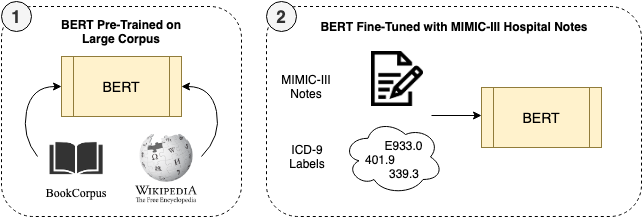
\includegraphics[width=0.8\linewidth]{bert_implementation_overview.jpeg}
\caption{ Overview of BERT implementation.}
\label{fig:view}
\end{figure}


\subsection{Experimental Setup}
We used Spark on Google Cloud Platform (GCP) via PySpark in a Python environment for data preprocessing. Implementing BERT requires a minimum of 16GB VRAM, which we utilized through a Deep Learning Platform release image on a GCP instance with 8 vCPUs, 58GB RAM and an NVIDIA Tesla P4 GPU. It is worth noting that pre-training BERT from scratch is a computationally expensive task, so we benefit greatly from using the existing pre-trained, open-source BERT model. 

\section{Experimental Results \& Discussion}
The CAML model achieved AUC-micro for CAML about 0.91. Our goal was to beat it.

As our first step, we ran BERT using using sequences with a maximum length of 128. We achieved 90\% evaluation accuracy and 0.83 Micro-F1 score on a top 50 label set after just a single epoch.

Our next step is to run BERT using sequences with a maximum length of 512. We will also  run a comparison between the truncated records used for our BERT model versus the same IDs fed through CAML’s preprocessing and run a comparison of the metrics to examine our model’s performance more directly.

Finally, we will discuss here the impact that the word sequence length has on the performance of the model. If the selected length is too short, then meaningful information is likely to be truncated; however, it is not necessarily true that longer sequence lengths will net a better performance (Devlin et al).


\section{Conclusion}
TODO


\bibliographystyle{plain}
\bibliography{biblio}

\end{document}